
\section{Тест производительности}

Для тестов я использвал утилиту gnuplot для построения графиков зависимости времени работы программы от величины числа. Так же для сравнения использовал библиотеку chrono для замера времени.

\begin{figure}[h]
  \begin{center}
    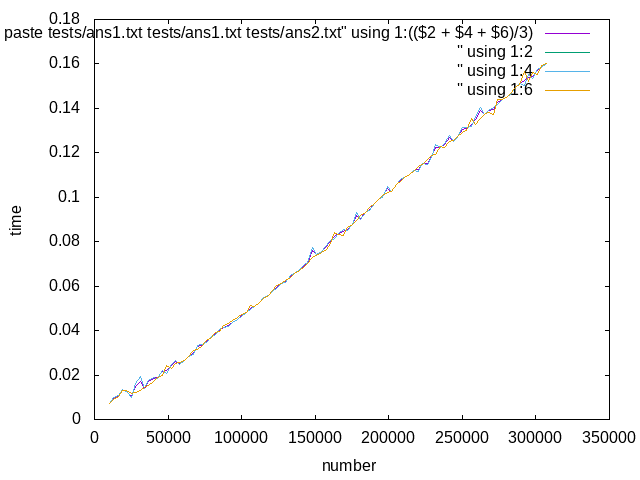
\includegraphics[scale=0.8]{../plots/plot1.png}
  \end{center}
  \caption{График времени работы поиска компонент связности от суммы количества вершин и ребер}
\end{figure}

Как мы можем заметить на Рис. 1 время работы алгоритма линейно зависит от суммы колличества вершин и ребер.

\pagebreak
